\chapter{Descrizione dello stage}
\label{cap:descrizione-stage}

In questo capitolo, viene fornita una spiegazione più dettagliata del progetto e della relativa organizzazione.

\section{Introduzione al progetto}

Uno dei principali mercati dove opera Euronovate è il mercato dei device di firma grafometrica
dotati di un monitor da 10 pollici multi-touch.\\ Questi dispositivi USB possono essere utilizzati
per molteplici scopi oltre all'inserimento di una firma in un documento, nel tempo l'azienda ha visto
realizzare sistemi di presentazioni slideshow, digital signage, questionari di valutazione e form
per l'aggiornamento delle anagrafiche.\\ Oggi Euronovate vuole spingersi ulteriormente nel mondo dei
multimedia e utilizzare il device di firma ENSign 11 per l'intrattenimento videoludico.\\

\section{Requisiti e obiettivi}

L'obiettivo dello stage è apprendere le nozioni dello sviluppo di applicazioni desktop e di integrazioni di dispositivi fisici, seguendo una pianificazione
settimanale delle attività.\\
Tale obiettivo viene raggiunto attraverso la realizzazione di un prodotto software, dall'analisi dello stesso alla sua validazione, passando per progettazione, codifica e collaudo.\\
In particolare, viene richiesto che il prodotto funzioni su un ambiente desktop e tramite il device di firma collegato allo stesso. Il device stesso è l'unico strumento di interazione con il software.\\
Viene quindi richiesto che il prodotto da sviluppare, ovvero ENGaming:
\begin{itemize}
    \item permetta il caricamento di giochi.
    \item permetta l'interazione con i giochi attraverso un controller virtuale, visibile nel device di firma.
    \item permetta la realizzazione, il salvataggio e la visione, dei punteggi effettuati nei singoli giochi.
\end{itemize}
Inoltre, per motivi aziendali, si vorrebbe che il prodotto richiesto possa essere eseguito indipendentemente dalla piattaforma, ovvero si vuole che il prodotto possa essere definito multipiattaforma.\\
Ulteriori feature di prodotto possono essere proposte, con valutazione da parte del tutor.

\section{Pianificazione}

\subsection{Fasi e dettagli}

In accordo con il tutor aziendale, si è deciso di suddividere il tirocinio nelle seguenti fasi:
\begin{itemize}
    \item Conoscenze generali, dal 2 Maggio al 5 Maggio.
    \item Formazione personale, dal 8 Maggio al 19 Maggio.
    \item Analisi dei Requisiti, dal 22 Maggio al 25 Maggio.
    \item Progettazione Tecnica, dal 25 Maggio al 2 Giugno.
    \item Codifica, dal 5 Giugno al 6 Luglio.
    \item Documentazione, dal 7 Luglio al 10 Luglio.
    \item Demo, l'11 Luglio.
\end{itemize}

\subsubsection{Conoscenze generali}
Questa fase, della durata di 4 giorni, prevede l'installazione degli ambienti di sviluppo e di versionamento, nonchè un approfondimento degli stessi. Inoltre, vengono abilitati gli strumenti aziendali (account git, AWS, Verdaggio e GSuite) necessari per il tirocinio.
\subsubsection{Formazione personale}
In questa fase, durata 10 giorni, l'obiettivo è l'approfondimento dello sviluppo attraverso le tecnologie necessarie per il progetto.\\
In particolare, l'approfondimento riguarda \gls{elctr} per lo sviluppo dell'applicazione desktop, comprese le tecniche di comunicazione tra processi per il passaggio dei dati tra \gls{cpp} e \gls{tsc}. Inoltre, è necessario approfondire il funzionamento del framework \gls{angl} per la parte front-end dell'applicativo.\\
L'approfondimento di questa fase produce una piccola applicazione che unisce tutte le parti appena citate.
\subsubsection{Analisi dei Requisiti}
Durante questa fase, della durata di 4 giorni, è necessaria per definire gli utenti che utilizzano l'applicativo e i casi d'uso che l'applicazione deve prevedere.\\
Inoltre, vengono elencati i requisiti che l'applicativo deve rispettare (dicasi requisiti obbligatori) e i requisiti che l'applicativo può rispettare (detti requisiti opzionali).\\
Tale analisi è alla base dell'intero sviluppo del prodotto, poichè indica \textbf{cosa} deve fare il prodotto, perciò tale fase viene ritenuta conclusa all'approvazione del documento da parte del tutor.
\subsubsection{Progettazione tecnica}
Questa fase, con durata di 7 giorni, indica gli elementi che andranno a creare l'applicativo.\\
Più concretamente, questa fase rivela:
\begin{itemize}
    \item le classi che verranno utilizzate.
    \item l'architettura che il prodotto dovrà avere.
    \item gli elementi di design che il prodotto utilizzerà.
    \item eventuali file di configurazione, dove si deve elencarne anche la struttura.
\end{itemize}
La progettazione è cruciale, in quanto permette di non cambiare (o più realisticamente, di cambiare il meno possibile) gli elementi che compongono l'applicativo.\\
Per tal motivo, anche questa fase viene ritenuta conclusa all'approvazione del documento da parte del tutor.
\subsubsection{Codifica}
Questa fase, la più sostanziosa con la sua durata di 24 giorni, prevede la stesura del codice dell'applicativo, partendo da quanto prodotto nella fase precedente.\\
Durante la stesura del codice, le parti prodotte vengono verificate attraverso dei test, che possono essere sia manuali che automatizzati.\\
Verso la conclusione di questa fase, il prodotto viene collaudato e validato.
\subsubsection{Documentazione}
In questa fase, della durata di 2 giorni, si va a creare la documentazione necessaria per l'utilizzo e la manuntenzione del prodotto.\\
Per questo progetto, si devono produrre due documenti:
\begin{itemize}
    \item \textbf{Manuale dello Sviluppatore}, dove si elencano i passaggi per la preparazione dell'ambiente di sviluppo, i problemi noti e i possibili miglioramenti.
    \item \textbf{Manuale Utente}, dove si elencano i requisiti di sistema e le attività che si possono effettuare con l'applicativo.
\end{itemize}
\subsubsection{Demo}
In questa ultima fase, della durata di un giorno, viene mostrato all'azienda quanto prodotto.\\
Questa esposizione permette allo stagista di mostrare quanto prodotto, e all'azienda di valutarne possibili riscontri nei prodotti attuali o nei prodotti futuri.

\subsection{Supervisione e controllo}
Le prime fasi dello stage sono di preparazione alle competenze necessarie al corretto svolgimento
del progetto.\\
Gli allineamenti con il referente aziendale vengono svolti ad ogni termine di attività.\\
Durante la fase di analisi, progettazione e codifica, gli allineamenti sono quotidiani, mentre gli incontri per gli sprint Agile e per la pianificazione delle attività
sono a cadenza settimanale.
\subsection{Diagramma di Gantt}
\begin{figure}[!h] 
    \centering 
    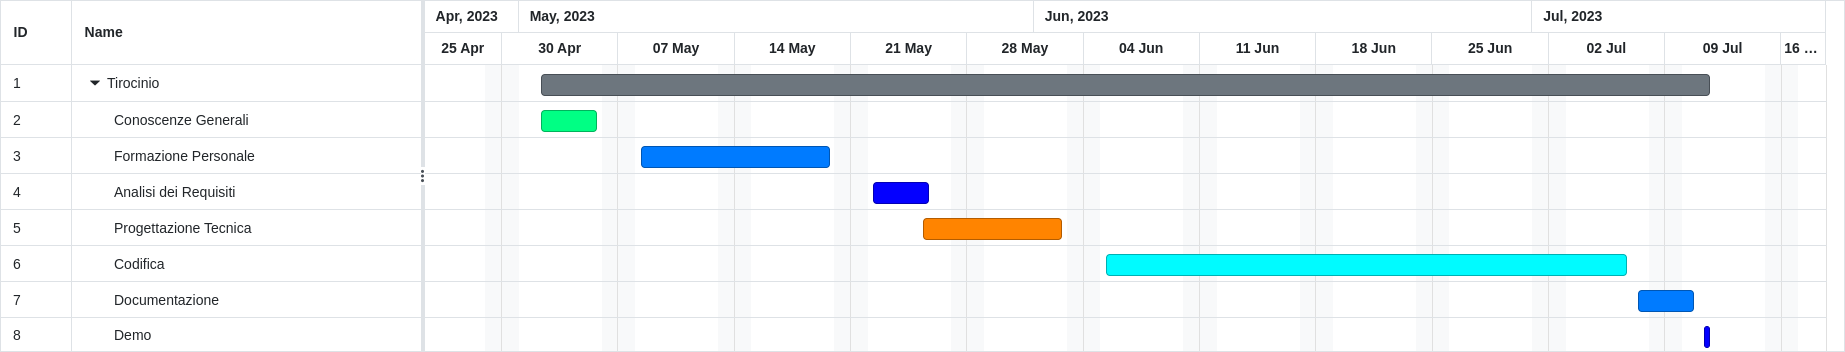
\includegraphics[width=350pt]{images/diagrammaGantt.png} 
    \caption{Diagramma di Gantt del tirocinio}
\end{figure}
